\documentclass{proc}
\usepackage[utf8]{inputenc}
\usepackage[english]{babel}
\usepackage{graphicx}
\usepackage{listings}
\usepackage{hyperref}
\usepackage{color}
\usepackage{textcomp}
\author{Eupharion, Zaero, Quis}
\title{It was a day}
\begin{document}
\maketitle
\section{Dataset and Models}
Dataset: MSCOCO\\
Two models were trained. The first model is the typical one that is introduced by Yunjey on github\footnote{\url{https://github.com/yunjey/pytorch-tutorial/tree/master/tutorials/03-advanced/image_captioning}}. 
\paragraph{} The captioning model utilises a CNN, an encoder, to encode the image, reducing it to its features. The features are then fed into the decoder network consisting of an LSTM, which then outputs the words accordingly.
\paragraph{} The models we utilised are built as follows:
\begin{enumerate}
\item Vgg 19 - batch norm, pretrained, frozen except last layer.
\item Linear layer, taking the place of the Vgg network's last layer. This linear layer is not frozen.
\item a Batch Normalisation layer after the linear layer.
\item an word embedding layer.
\item LSTM layer.
\item One final linear layer that maps the output to words.
\end{enumerate}

\subsection{Yunjey's model}
Yunjey's model involves concatenating the image and the captions as input during training and validation, attempting guide the outputs in a similar direction to purely training based off images and expecting an output which points to the correct caption. Validation is done in the same manner with the features concatenated with the captions to search for the right outputs. Sampling however, does not take in the caption as an additional parameter, with the decoder only taking in the original input.\\

\subsection{Alternative model}
The alternative model we propose is different in where the input from the encoder is fed into the network via the hidden state, and the input is simply a start token at the start. During training, the correct words from the $t_{-1}$ time step are fed into the input so as to guide the network into learning the relationship between the words appearances and the input hidden state. This was however a mistake on our part, as it leads to inefficient memory space usage. It is possible that feeding it into the hidden state at the start and expecting that the hidden state outputs the relevant output means that parameters have to be wasted, focused on translating the relevant information into the cell state instead of the approximating the correct word into the output hidden state for the next cycle as opposed to purely basing itself off the existing cell states. In other words, we placed the data into the output area (hidden state)instead of the vector that was directly reserved for memory (cell state). While the neural network was able to adapt, it might have impacted performances negatively.
\begin{enumerate}
\item 
\end{enumerate}
\section{Hyper parameter choices}
The following hyper parameters were used for both models initially.
\begin{itemize}
\item total epochs = 30
\item embedding size = 50 
\item learning rate = 0.001 
\item momentum = 0.9
\item number of layered LSTMs = 2
\item number of hidden dimensions in LSTM = 300
\item Loss function = CrossEntropyLoss
\item decay rate = 0.9 (Multiplier applied with every epoch end)
\item training transforms:
\begin{lstlisting}[language = python]
from torchvision import transforms
transforms.Compose([
transforms.Resize(300), 
transforms.RandomCrop(224), 
transforms.RandomHorizontalFlip(),
transforms.ToTensor(), 
transforms.Normalize(
(0.485, 0.456, 0.406),
(0.229, 0.224, 0.225))])
\end{lstlisting}
\item testing transforms:
\begin{lstlisting}[language = python]
transforms.Compose([ 
transforms.Resize(224),
transforms.CenterCrop(224),
transforms.ToTensor(), 
transforms.Normalize(
(0.485, 0.456, 0.406),  
(0.229, 0.224, 0.225))])
\end{lstlisting}
\item batchsize = 32/16/8
\end{itemize}
\paragraph{} Batch sizes were altered as we began to experiences plateaus in training, validation and sampling performance. Each time the batch size is altered to become smaller, we force the gradient to update along smaller numbers of features. This slows training somewhat due to the increased number of batch propagations, but due to the larger number of updates, the gradient is forced to learn even more specific features from each batch with every iteration. Because the model is forced to learn even more features with each iteration, the space in which the local minima was originally constructed changes, with the ability to capture even more features to further decrease loss rate is enhanced.
\paragraph{} Batch sizes were altered for the model based off Yunjey's example as follows: 32 till epoch number 8, halved to 16 till epoch 15 before being halved one more time to 8.
\paragraph{} Batch sizes for our alternative model stayed at 32 except for the last 2 epochs where it was switched to 16. However, there are several complications in our training process.
\section{Word frequency analysis}
\begin{figure}[h!]
  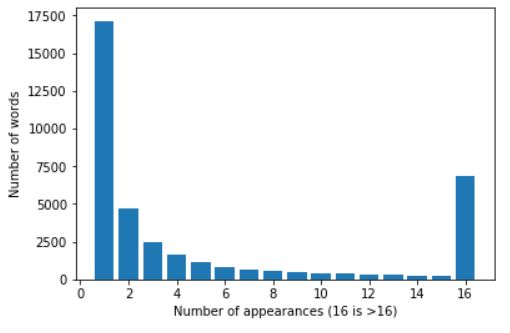
\includegraphics[width=\linewidth]{barchar.JPG}
\end{figure}
As seen in the bar chart above, where the 16th category is the number of words that have more then 16 appearances in the entire dataset, a majority of words do not appear more then once (17150 words). This is a significant majority of words since there are only a total of 38406 unique words in the dataset. As a result, we opt not to edit the dataset in our training, using those words as part of the training or validation data accordingly. This is because we believed it would result in a large amount of the unknown word token showing up in the training set, heavily impacting performance. 
\section{Evaluation}

\section{Packages used}
\begin{enumerate}
\item NLTK - version 3.4 \\
You will need to also run 
\begin{lstlisting}[language=python]
nltk.download('punkt')
\end{lstlisting}
In your python file (NOT IN SHELL)
\end{enumerate}

\end{document}
